%% arara directives
% arara: xelatex
% arara: bibtex
% arara: xelatex
% arara: xelatex

\documentclass{article} % One-column default
%\documentclass[twocolumn, switch]{article} % Method A for two-column formatting

\usepackage{preprint}
\usepackage{natbib}
%% Math packages
\usepackage{amsmath, amsthm, amssymb, amsfonts}

%% Bibliography options
%\usepackage[numbers,square]{natbib}
%\bibliographystyle{unsrtnat}
%\usepackage{apacite}
%\usepackage{natbib}
%\bibliographystyle{Geology}
\bibliographystyle{cas-model2-names}

%% General packages
\usepackage[utf8]{inputenc}	% allow utf-8 input
\usepackage[T1]{fontenc}	% use 8-bit T1 fonts
\usepackage{xcolor}		% colors for hyperlinks
\usepackage[colorlinks = true,
            linkcolor = purple,
            urlcolor  = blue,
            citecolor = cyan,
            anchorcolor = black]{hyperref}	% Color links to references, figures, etc.
\usepackage{booktabs} 		% professional-quality tables
\usepackage{nicefrac}		% compact symbols for 1/2, etc.
\usepackage{microtype}		% microtypography
\usepackage{lineno}		% Line numbers
\usepackage{float}			% Allows for figures within multicol
\usepackage{multicol}		% Multiple columns (Method B)

\usepackage{lipsum}		%  Filler text

 %% Special figure caption options
\usepackage{newfloat}
\DeclareFloatingEnvironment[name={Supplementary Figure}]{suppfigure}
\usepackage{sidecap}
\sidecaptionvpos{figure}{c}

% Section title spacing  options
\usepackage{titlesec}
\titlespacing\section{0pt}{12pt plus 3pt minus 3pt}{1pt plus 1pt minus 1pt}
\titlespacing\subsection{0pt}{10pt plus 3pt minus 3pt}{1pt plus 1pt minus 1pt}
\titlespacing\subsubsection{0pt}{8pt plus 3pt minus 3pt}{1pt plus 1pt minus 1pt}

% ORCiD insertion
\usepackage{tikz,xcolor,hyperref}

\definecolor{lime}{HTML}{A6CE39}
\DeclareRobustCommand{\orcidicon}{
	
\begin{tikzpicture}
	\draw[lime, fill=lime] (0,0) 
	circle [radius=0.16] 
	node[white] {{\fontfamily{qag}\selectfont \tiny ID}};
	\draw[white, fill=white] (-0.0625,0.095) 
	circle [radius=0.007];
	\end{tikzpicture}
	\hspace{-2mm}
}
\foreach \x in {A, ..., Z}{\expandafter\xdef\csname orcid\x\endcsname{\noexpand\href{https://orcid.org/\csname orcidauthor\x\endcsname}
			{\noexpand\orcidicon}}
}
% Define the ORCID iD command for each author separately. Here done for two authors.
\newcommand{\orcidauthorA}{0000-0002-8124-7536}
\newcommand{\orcidauthorB}{0000-0003-4252-7161}
\newcommand{\orcidauthorC}{0000-0002-7647-6852}


%%%%%%%%%%%%%%%%   Title   %%%%%%%%%%%%%%%%
\title{A data-driven framework for paleomagnetic Euler pole analysis}

% Add watermark with submission status
%\usepackage{xwatermark}
% Left watermark
%\newwatermark[firstpage,color=gray!60,angle=90,scale=0.32, xpos=-4.05in,ypos=0]{\href{https://doi.org/}{\color{gray}{Publication doi}}}
% Right watermark
%\newwatermark[firstpage,color=gray!60,angle=90,scale=0.32, xpos=3.9in,ypos=0]{\href{https://doi.org/}{\color{gray}{Preprint doi}}}
% Bottom watermark
%\newwatermark[firstpage,color=gray!90,angle=0,scale=0.28, xpos=0in,ypos=-5in]{*correspondence: \texttt{email@institution.edu}}

%%%%%%%%%%%%%%%  Author list  %%%%%%%%%%%%%%%
\usepackage{authblk}
\renewcommand*{\Authfont}{\bfseries}
\author[1\thanks{\tt{l.c.gallo@geo.uio.no}}]{Leandro C. Gallo\orcidA{}}
\author[2]{Facundo Sapienza\orcidB{}}
\author[1]{Mathew Domeier\orcidC{}}

\affil[1]{Centre for Earth Evolution and Dynamics, University of Oslo, Norway}
\affil[2]{Department of Statistics, University of California Berkeley, United States}

% Option 2 for author list
%\author{
%  David S.~Hippocampus\thanks{Use footnote for providing further
%    information about author (webpage, alternative
%    address)---\emph{not} for acknowledging funding agencies.} \\
%  Department of Computer Science\\
%  Cranberry-Lemon University\\
%  Pittsburgh, PA 15213 \\
%  \texttt{hippo@cs.cranberry-lemon.edu} \\
%  %% examples of more authors
%   \And
% Elias D.~Striatum \\
%  Department of Electrical Engineering\\
%  Mount-Sheikh University\\
%  Santa Narimana, Levand \\
%  \texttt{stariate@ee.mount-sheikh.edu} \\
%  \AND
%  Coauthor \\
%  Affiliation \\
%  Address \\
%  \texttt{email} \\
%  % etc.
%}

%%%%%%%%%%%%%%    Front matter    %%%%%%%%%%%%%%
\begin{document}

%\twocolumn[ % Method A for two-column formatting
  \begin{@twocolumnfalse} % Method A for two-column formatting
  
\maketitle

\begin{abstract}
Owing to the inherent axial symmetry of the Earth’s magnetic field, paleomagnetic data only directly record the latitudinal and azimuthal positions of crustal blocks in the past, but paleolongitude cannot be constrained. An ability to overcome this obstacle is fundamental to paleogeographic reconstruction. The paleomagnetic Euler pole (PEP) analysis presents a unique means to recover such information in deep-time. However, prior applications of the PEP method have invariably incorporated subjective decisions into its execution, undercutting its fidelity and rigor. Here we present a data-driven approach to PEP analysis that addresses some of these deficiencies---namely the objective identification of change-points and small-circle arcs that together approximate an apparent polar wander path. We elaborate on our novel methodology and conduct some experiments with synthetic data to demonstrate its performance. We furthermore present implementations of our methods both as adaptable, stand-alone scripts and as a streamlined interactive workflow that can be operated through a web browser.
\end{abstract}
%\keywords{First keyword \and Second keyword \and More} % (optional)
\vspace{0.35cm}

  \end{@twocolumnfalse} % Method A for two-column formatting
%] % Method A for two-column formatting

%\begin{multicols}{2} % Method B for two-column formatting (doesn't play well with line numbers), comment out if using method A


%%%%%%%%%%%%%%%  Main text   %%%%%%%%%%%%%%%
% \linenumbers

\section{Introduction}
Following from Euler's rotation theorem (or fixed point theorem), the motions of lithospheric plates across the surface of the sphere can be precisely described in the form of finite rotations---commonly called Euler vectors (or Euler poles)---which can be concisely expressed by three parameters: the latitude and longitude of a pole of rotation $(\theta, \phi)$ and an angular displacement $\psi$. In plate tectonic and paleogeographic research, great effort is dedicated toward unraveling and chronicling the history of plate kinematics, which is tantamount to the determination and collation of Euler vectors. Improvements and innovations in the methods of Euler vector inference are therefore of broad importance.

An assumption common to all methods of Euler vector inference is that the motion of a given plate with respect to some arbitrary reference can be treated as stable over some nominal interval, such that it can be expressed by a single 'stage' Euler vector \citep{gordon1984paleomagnetic, cox1986plate}. From the perspective of the system of reference, this stage Euler vector will be fixed and any point belonging to the plate will move along a plane perpendicular of that axis of rotation, tracing a circle centered on it. If an object passes from the domain of the reference to the plate (becoming a passive occupant of the latter), it too will follow the path of a circle during the stage interval, with a displacement proportional to its residence time on the plate. A series of such objects, passed from the reference domain to the plate progressively in time during the stage interval, would therefore form an arcuate array decorating the trace of a circle about the Euler vector. If a sufficient number of such objects could be identified, their distribution could be inverted to retrieve the location of the Euler vector, and their corresponding residence times on the plate could be used to determine its amplitude $\psi$.

At least two kinds of observational records present such age-progressive arcuate segments that can be used to infer stage Euler vectors: hotspot tracks and paleomagnetic apparent polar wander paths (APWPs) (Figure \ref{fig:intro_cartoon}). Hotspot tracks record the motion of a plate with respect to the underlying mantle, whereas APWPs record the motion of a plate relative to the Earth's magnetic field, which is aligned with the planetary rotation axis. The inversion of paleomagnetic data to retrieve stage Euler vectors---or paleomagnetic Euler pole (PEP) analysis---is of particular interest because it offers the possibility to recover full kinematic descriptions of past plate motion, in contrast to the conventional analysis of paleomagnetic data, which constrains only paleolatitude and paleoazimuth. However, despite being first conceptually introduced more than half a century ago \citep{francheteau1969paleomagnetism}, PEP analysis has seen limited application \citep[e.g.][]{smirnov2010co,wu2017absolute,swanson2019failed,beck2003absolute, gordon1984paleomagnetic}. This appears to be due, at least in part, to the fact that most prior approaches to PEP analysis have incorporated subjective decisions into its execution. In order to secure the reproducibility of scientific results, our objective here is to introduce an unsupervised and objective framework with which to conduct PEP analysis---although our methodology is applicable to stage Euler vector inference more generally. We furthermore seek to provide an accessible implementation of this framework for community use by the use of Jupyter notebooks \citep{Kluyver:2016aa} that can be easily deployed using Binder \citep{project_jupyter-proc-scipy-2018}.

\begin{figure}
\begin{centering}
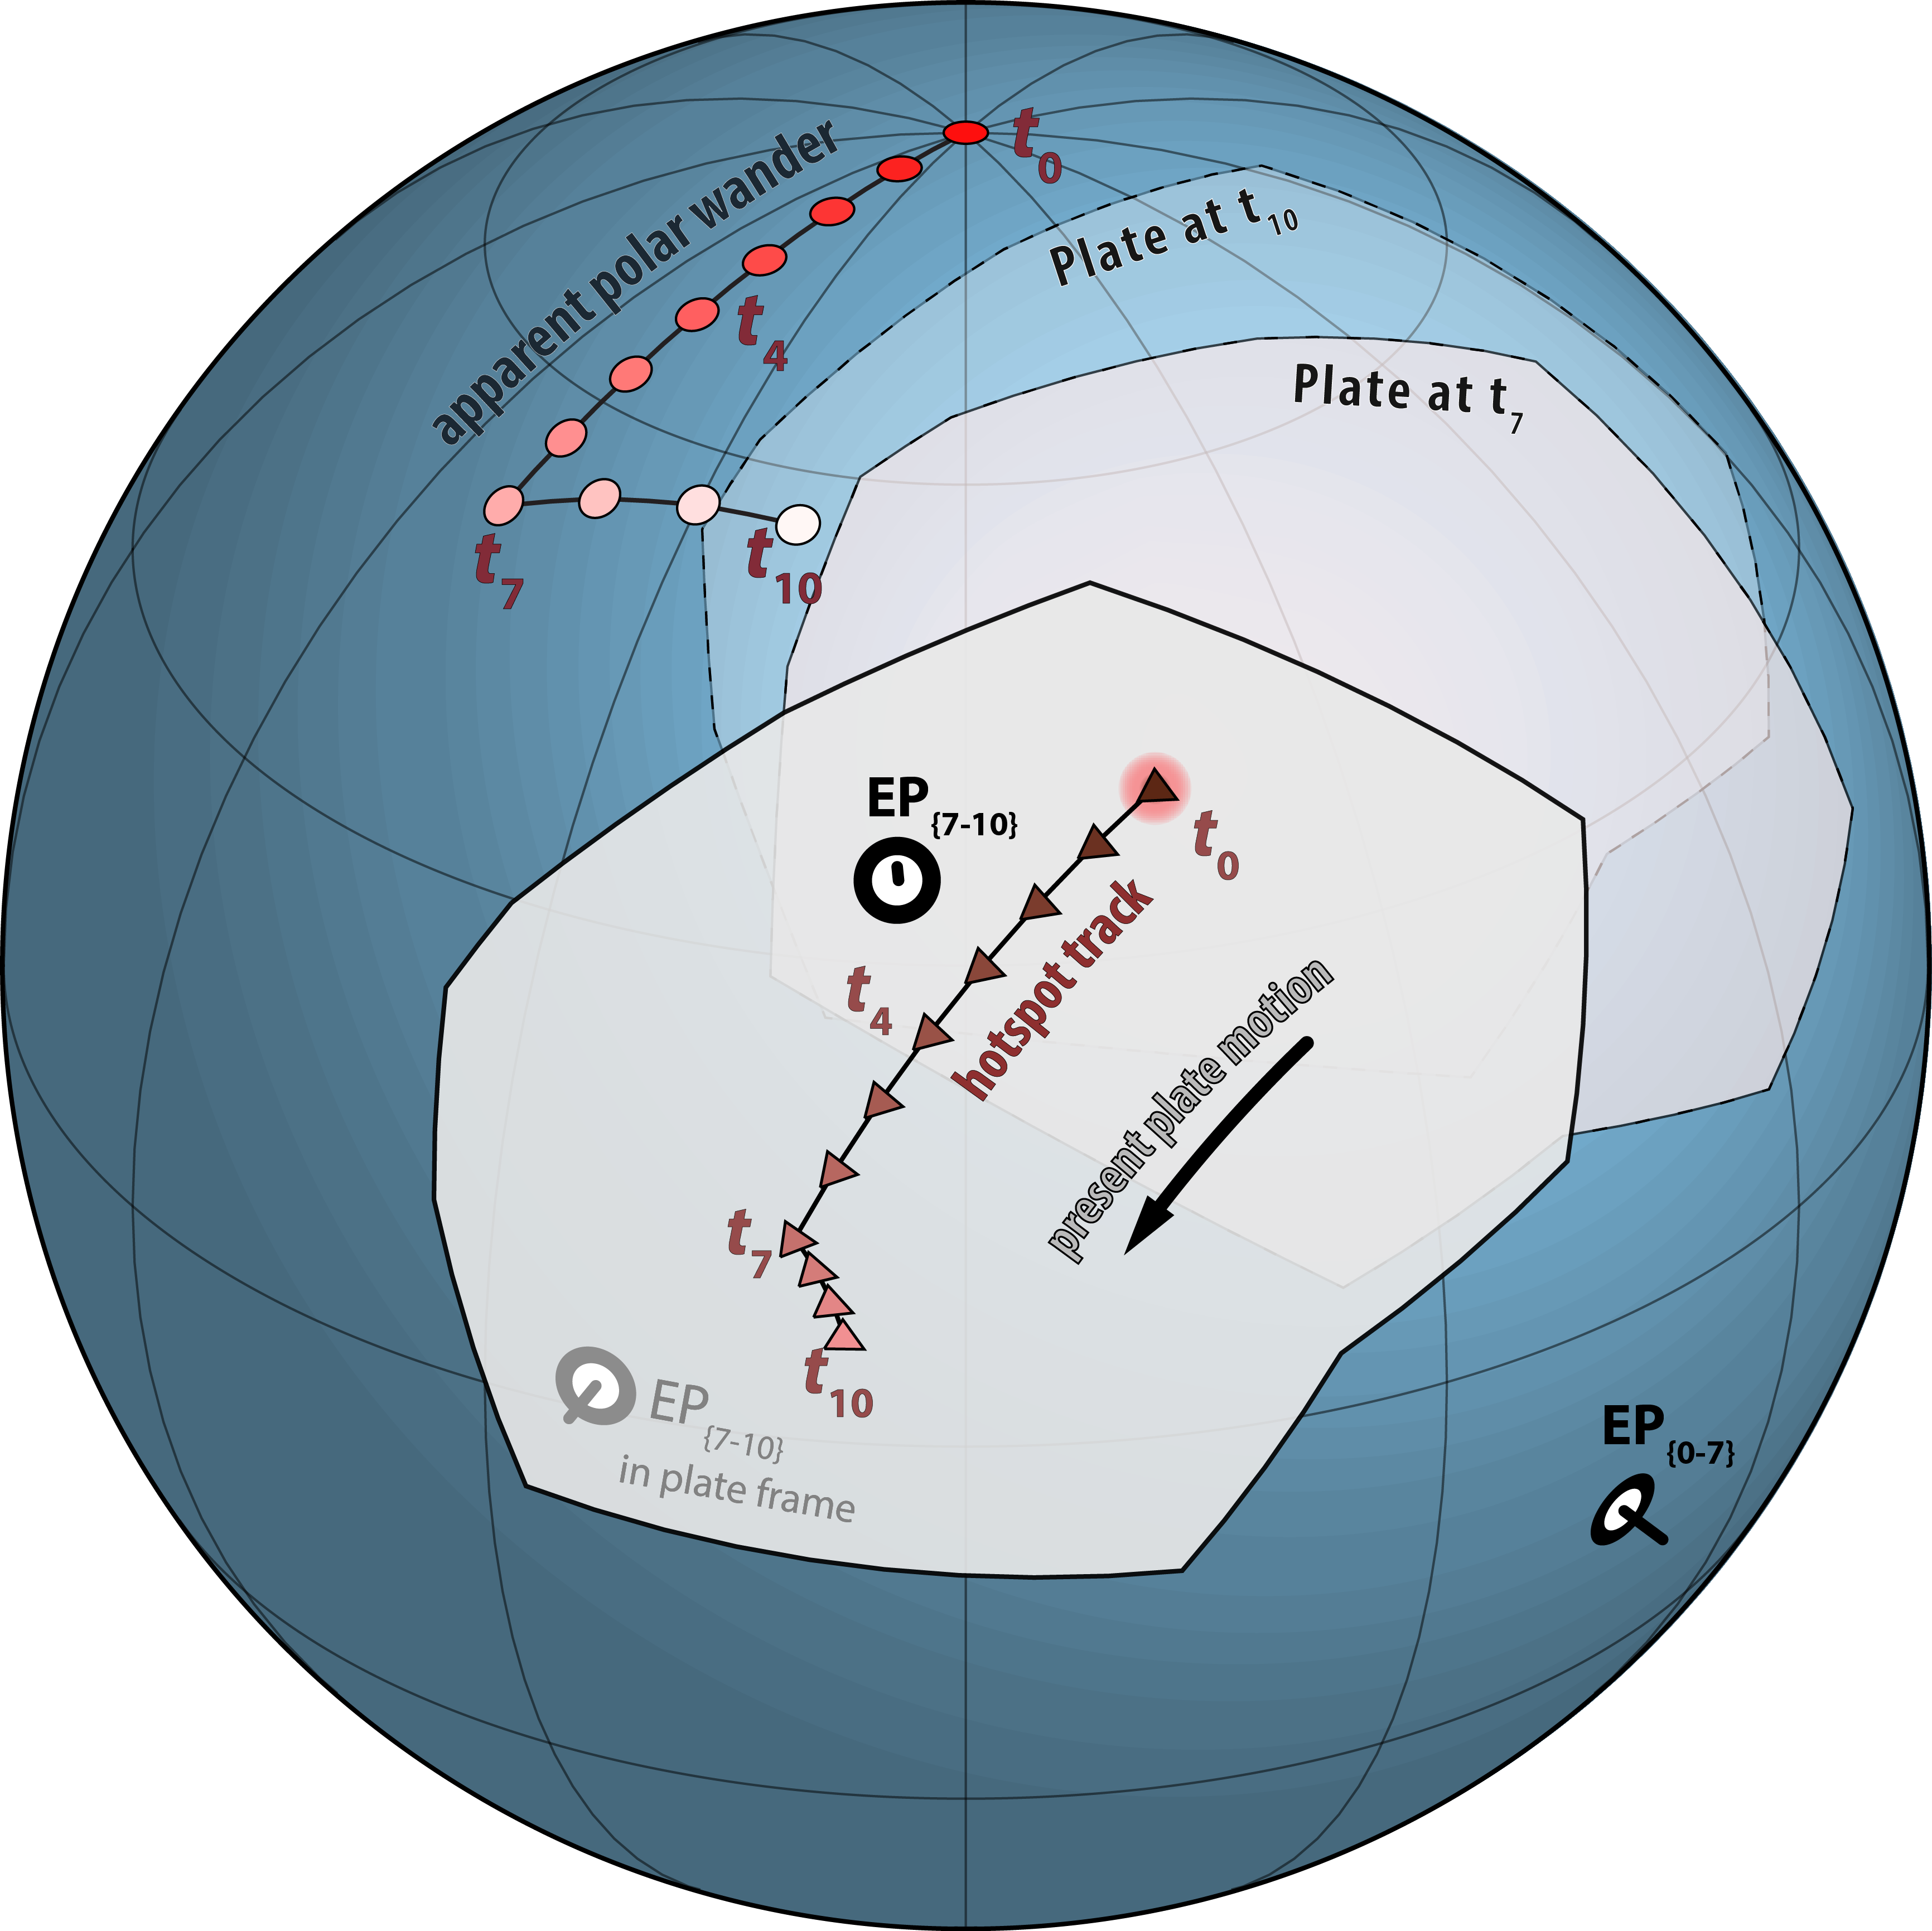
\includegraphics[scale=0.25]{intro_cartoon.png}

\caption{\small Cartoon illustrating the relationship between an apparent polar wander path (APWP; blue circles), a hotspot track (red triangles) and the Euler poles (EP; black poles) describing the kinematics of the host plate (grey polygon with static boundaries for simplicity) which gave rise to them over some interval of time ($t_0$-$t_{10}$). A sequence of paleomagnetic poles and/or hotspot volcanoes may be inverted to discover the location of the corresponding EP.}

\label{fig:intro_cartoon}
\end{centering}
\end{figure}

\section{Paleomagnetic Euler pole analysis}

If a given plate's motion relative to the planetary spin-axis is constant for some interval of time, the paleomagnetic poles aquired by the plate over that interval will trace an arc across the surface of the sphere. The fundamental task in PEP analysis is to invert an assemblage of paleomagnetic data to retrieve the average instantaneous kinematics that were acting during such an interval (i.e. the stage Euler vector). However, because plate motions intermittently change according to force balance adjustments, APWPs comprise a discrete series of arcuate segments separated by change-points whose number and timing is unknown. Thus, PEP analysis also necessitates the division of paleomagnetic data into a number of temporal subsets--or groups--such all the paleomagnetic poles of a given group represent the same (unknown) stage Euler vector. We are thus presented with two tasks that we may treat as distinct optimization problems:

\begin{enumerate}
    \item Grouping paleomagnetic data into subsets that manifest distinct stage Euler vectors.
    \item Determination of the best-fit stage Euler vector for each paleomagnetic subset.
\end{enumerate}

Here we develop an unsupervised search process to solve these problems in the reverse order by first determining the best-fit stage Euler vector to all possible APWP segments (all ordered subsets of the paleomagnetic data), and then identify the least-cost sequence of Euler vectors approximating the total APWP. 

\section{Methodology}

We start by considering that we have a series of $N$ paleomagnetic poles that we call $p_i$, whit $i = 1, 2, \ldots, N$. Each one of these paleomagnetic poles have an associated date $t_i$ and can be represented in Cartesian coordinates $(x_i, y_i, z_i)$---with $x_i^2 + y_i^2 + z_i^2 = 1$---and also by their latitude and longitude, $(\theta_i, \phi_i)$. Without loss of generality, we assume that the paleomagnetic poles are time ordered, meaning $t_i < t_j$ for $i < j$. We refer to $P = \{ p_1, p_2, \ldots, p_N \}$ as the full sequence of paleomagnetic poles that defines the APWP. Furthermore, given two indices $i$ and $j$ with ${i < j}$, we denote by $P_{i-j} = \{ p_i, p_{i+1}, \ldots, p_{j}\}$ the subsequence of paleomagnetic points contained in the interval of time between $t_i$ and $t_j$. We use $q$ to refer to Euler poles, where $q_i$ is the instantaneous Euler pole at time $t_i$. Lastly, we denote with $R(q, \omega)$ the matrix describing a rigid counterclockwise rotation around the axis $q$ by the angle $\omega$, which thus represents the average instantaneous rotation over the time interval---or stage---i.e. a stage Euler vector.

\subsection{Gradient-based Euler vector optimization from paleomagnetic data}

In this section we consider the problem of fitting an arc (whether belonging to a small- or great-circle) to a subsequence of paleomagnetic poles. Given $k$ and $m$ with $k< m$, we want to find the coordinates of the Euler pole $q$ and an angle $\varphi \in [0, \pi / 2]$ such that the points in $P_{k-m}$ are approximated by the trace of a circle with angular radius $\varphi$, centered on Euler pole $q$ (Figure \ref{fig:circle_fitting}a).

\begin{figure}
\begin{centering}
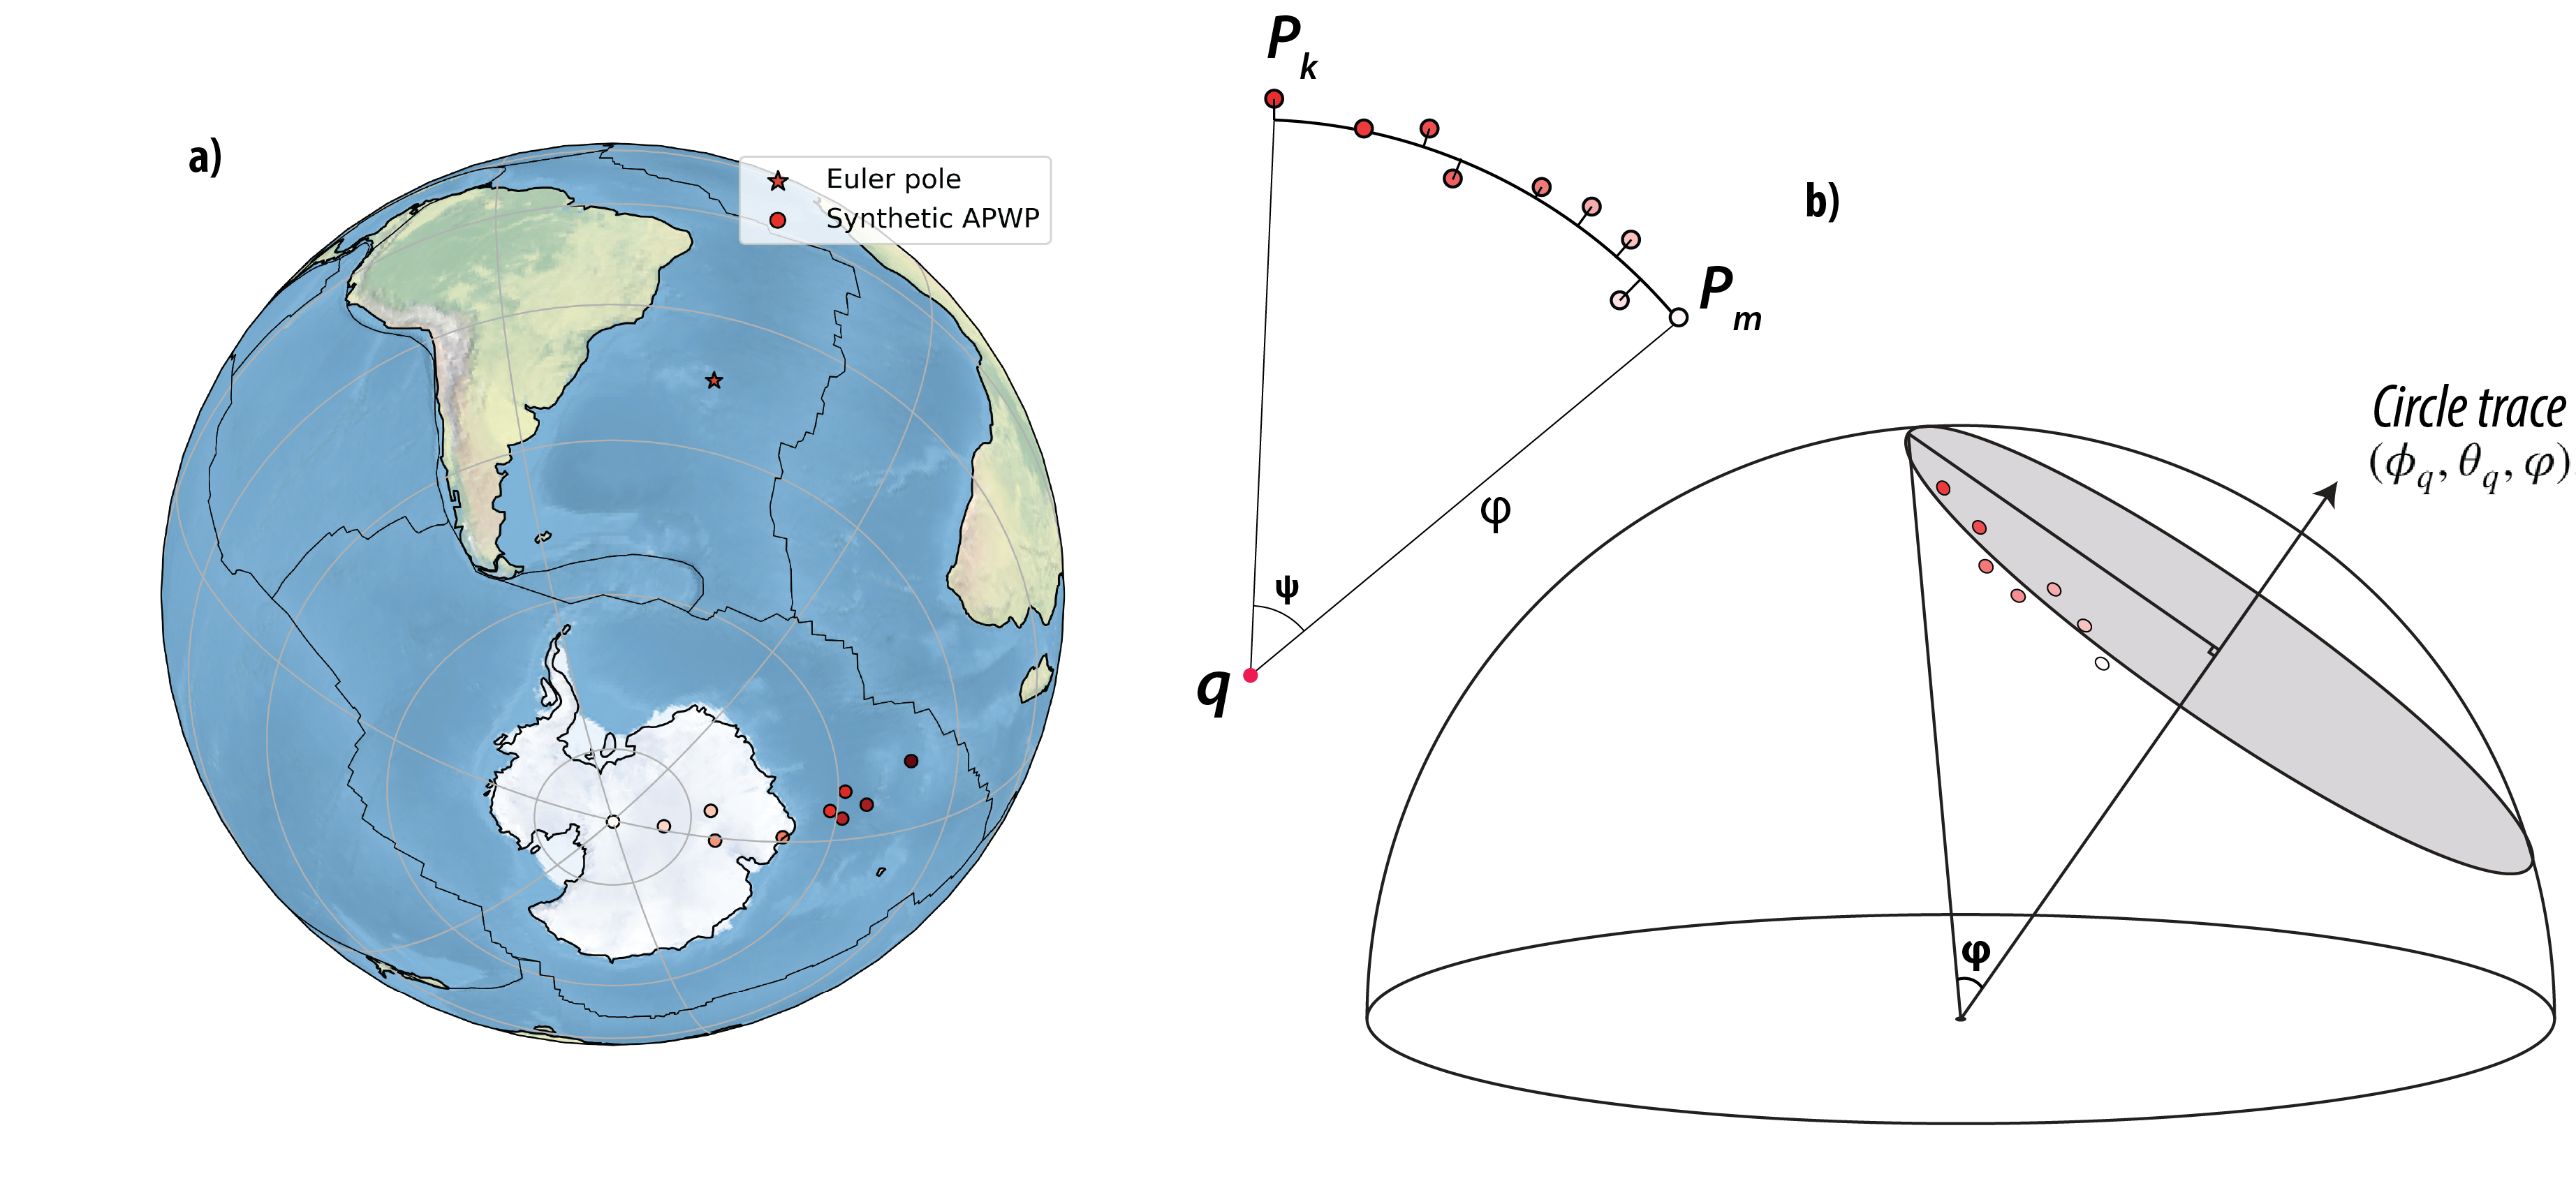
\includegraphics[scale=0.5]{Figure 2.png}

\caption{\small a) Orthographic representation of a synthetic sequence of paleomagnetic poles (generated by supplementary Jupyter Notebook -- Gradient-based\_Euler\_optimization.ipynb). b) Schematic representation of the optimized Euler vector to the same orientation data}

\label{fig:circle_fitting}
\end{centering}
\end{figure}

We infer the parameters of the circle by minimizing the sum of the squares of the geodesic distance from each data point to the circle trace. The geodesic distance can be computed as the absolute difference of the angle between the Euler pole $q$ and each paleomagnetic pole $p_i$ and the angle $\varphi$:
\begin{equation}
    \text{geod}(p_i; q, \varphi) = \left | \cos^{-1}(x_i x_q  + y_i y_q + z_i z_q) - \varphi  \right |,
\end{equation}
with $(x_q, y_q, z_q)$ the coordinates of the Euler pole $q$.
Then, we consider an optimization problem that seeks to minimize the cost function given by 
\begin{equation}
    \mathcal C_{k-m} (\Theta) = \sum_{i=k}^{m} \text{geod}(p_i; q, \varphi )^2,
    \label{costfunction}
\end{equation}
where the optimization is perform with respect to the three parameters of the circle that we write as the three-dimensional vector $\Theta = (\theta_q, \phi_q,  \varphi )$. In the noiseless case where all the points lie along a small- or great-circle and satisfy the equation $x x_q + y y_q + z z_q = \cos \varphi$ for all $p \in P_{k-m}$, the quantity $\mathcal{C}_{k-m}(\Theta)$ achieves its minimum at zero. Since each $(x_i, y_i, z_i)$ is typically affected by random perturbations, there is no exact fit between the set of points and a small or great circle trace.  

In contrast to the ordinary least squares method, this optimization problem has no analytical solutions. Although an optimal solution can be found numerically via grid searching \citep[e.g.][]{gordon1984paleomagnetic}, such an approach converges slowly.  This approach was also considered in \cite{gray1980} and \cite{fujiki2009}, where the authors use a constrained optimization method to find the Cartesian coordinates of the pole. 
Here we employ the nonlinear conjugate gradient method of \citet{polak1969note} to find an optimal solution more efficiently. %The conjugate gradient algorithm computes the gradient of the cost function and updates model parameters through $N_{iter}$ descent steps. For each learning step in $n = 0, 1, 2, \ldots, N_{iter} - 1$, the value of a random trial vector of initial parameters $\Theta_0$ is updated based on the update rule $\Theta_{n+1} = \Theta_n - \eta_n \nabla \mathcal C (\Theta_n)$, with $\nabla \mathcal C (\Theta_n)$ the gradient of $\mathcal C$ evaluated at $\Theta_n$, and $\eta_n$  the learning rate controlling the step size of each learning step. 
We take advantage of the solver provided in the open-source SciPy package \citep{virtanen2020scipy} to perform the computations. 
%This approach was also considered in \cite{gray1980} and \cite{fujiki2009}, but here we directly optimize on the angles instead of on the Cartesian coordinates of the pole, allowing us to omit constraints. 
It is worth noting that even though we have the following constraints $\theta_{q} \in [0, \pi]$, $\phi_{q} \in [0, 2\pi )$ and $\varphi \in [0, \pi)$, the periodicity of the cosine and sine functions allow us to treat this problem as an optimization problem without constraints.

The final update yields a single Euler pole which best describes the subsequence of paleomagnetic poles (Figure \ref{fig:circle_fitting}b). Its cost function gives the sum of the residuals between the predicted and observed paleomagnetic poles, and thus, a measure of goodness of fit. Using the spherical law of cosines, from the geographic coordinates of the inverted Euler pole $(\theta_q, \phi_q)$ we can infer a stage rotation angle $\psi$, that is, the rotation angle needed to translate the youngest paleomagnetic pole $p_k$ to the oldest one $p_{m}$, at an average angular velocity $\omega = \psi / (t_{m-1} - t_k)$. To illustrate the performance of our methodology, an example Jupyter notebook with synthetic data is provided  via \textit{Binder} (\url{https://mybinder.org/v2/gh/LenGallo/PEPy/HEAD}).

\subsection{Identifying the least-cost sequence of Euler vectors approximating an APWP}

Equipped with a method to invert a given set of paleomagnetic data to recover the best-fitting Euler vector describing them, we now present a  method that seeks to identify the unknown change-points (i.e. plate-motion changes) that divide an APWP into discrete segments associated with distinct stage Euler vectors. This is accomplished by seeking that sequence of change-points and Euler vectors which maximizes the goodness of fit between the predicted and observed paleomagnetic poles.

Our goal is to identify a subsequence of ordered indices (i.e. change-points) $j_1, j_2, \ldots, j_{m+1}$, with $j_1 = 1$ and $j_{m+1} = N+1$, such that each one of the $m$ segments $P_{j_k - j_{k+1}}$ belongs to the same circle. This implies that $q^{(i)} = q_{j_1} = \ldots = q_{j_{i+1}-1}$ and $\varphi^{(i)} = \varphi_{j_1} = \ldots = \varphi_{j_{i+1}-1}$ for all $k = 1, 2, \ldots, m$, where we define by $q^{(i)}$ and $\varphi^{(i)}$ the Euler pole and radius of the circle in the $i$th segment---or stage---of the APWP. In order to do so, we seek to minimize the following cost function 
\begin{equation}
    \min_{ \substack{ m, \, (j_1, j_2, \ldots, j_{m+1}), \\ (q^{(k)}, \varphi^{(k)})_{k=1}^m } } 
    \sum_{i=1}^N \text{geod}(p_i; q_i, \varphi_i)^2 + \lambda m,
    \label{eq:cost_2}
\end{equation}
where the optimization is performed over all possible increasing paths $(j_1, j_2, \ldots, j+m+1)$ of unknown length $m$ with $j_1=1$, $j_{m+1}=N+1$; and with respect to the Euler pole $q^{(k)}$ and rotation angle $\varphi^{(k)}$ associated to each one of the $m$ segments $P_{j_k-j_{k+1}}$.
%The number $m$ and timing of plate-motion changes that occur over the time interval represented by the APWP are treated as unknowns.
The last term $\lambda m$ in the cost function \eqref{eq:cost_2} corresponds to a regularization added to avoid overfitting, with $\lambda \geq 0$ a hyperparameter of the model. Large values of $\lambda$ will increase the value of the cost function, such that a good-fitting APWP with fewer segments will be favored. Note that equation \eqref{eq:cost_2} can be rewritten as
\begin{equation}
    \min_{  m, \, (j_1, j_2, \ldots, j_{m+1}) } 
    \sum_{k=1}^m \left( \min_{\Theta^{(k)}}  \mathcal C_{j_k - j_{k+1}}(\Theta^{(k)}) + \lambda \right),
    \label{eq:cost_3}
\end{equation}
with $\Theta^{(k)}$ the parameters of the minimum circle for the segment $P_{j_k - j_{k+1}}$. Based on the method introduced in section 3.1, we can find the Euler pole and amplitude for each one of the possible segments $P_{i-j}$ for each possible value of $i$ and $j$, and then compute the minimum inside the parentheses in equation \eqref{eq:cost_3}.

Our approach to minimize the cost function of equation \eqref{eq:cost_3} proceeds with an exploratory data analysis to characterize all possible pathways  $P_{i-j}$, and then employs a graph representation of the APWP to discover the optimal sequence of change-points $(j_1, j_2, \ldots, j_{m+1})$ and the number $m$ which yield the minimum sum of squared misfits between the set of paleomagnetic poles and the modelled arc segments describing them.

Graphs are compact mathematical structures that amount to a set of connected objects, where objects are referred to as nodes and connections are referred to as arrows (or edges for undirected graphs). Arrows can have an associated weight that indicates the cost of traversing them. An APWP can then be considered as a network where the nodes correspond to paleomagnetic poles and pairs of nodes are connected by arrows, to which a numerical weight can be assigned (Figure \ref{fig:graph}). We may thus model an APWP $P = \{ p_1, p_2, \ldots, p_N \}$ where the arrow from $p_i$ to $p_j$ exists for all $i, j$ such that $t_j > t_i$ and at least $3$ paleomagnetic poles (in order to define a plane, at least 3 non-colinear points are required). The weight of each arrow is given by the optimal value of the function $\mathcal C_{i-j}$ plus $\lambda$. In order to be consistent with our previous notation, the contribution of the last paleomagnetic pole $p_N$ is included in the weight of each arrow with its tail in $p_N$, that is, the weight of each arrow from $p_i$ to $p_N$ is given by the goodness of fit of the sequence $P_{i-(N+1)} = \{ p_i, \ldots, p_N \}$ plus $\lambda$. In this context, a candidate approximation of the APWP can be seen as the directed path $(p_{j_1}, p_{j_2}, \ldots, p_{j_{m+1}})$ with $p_{j_1} = p_1$ and $p_{j_{m+1}} = p_N$, where each pair of consecutive nodes in the path $(p_{j_k}, p_{j_{k+1}})$ is connected by an arrow. The total cost of each alternative series of directed paths is given by the sum of the individual weights of the arrows in the path, which coincides with equations \eqref{eq:cost_2} and \eqref{eq:cost_3}. The characterization of all possible pathways $P_{i-j}$ is accomplished by a moving window searching algorithm, where each possible $P_{i-j}$ is analyzed. 

\begin{figure}
\begin{centering}
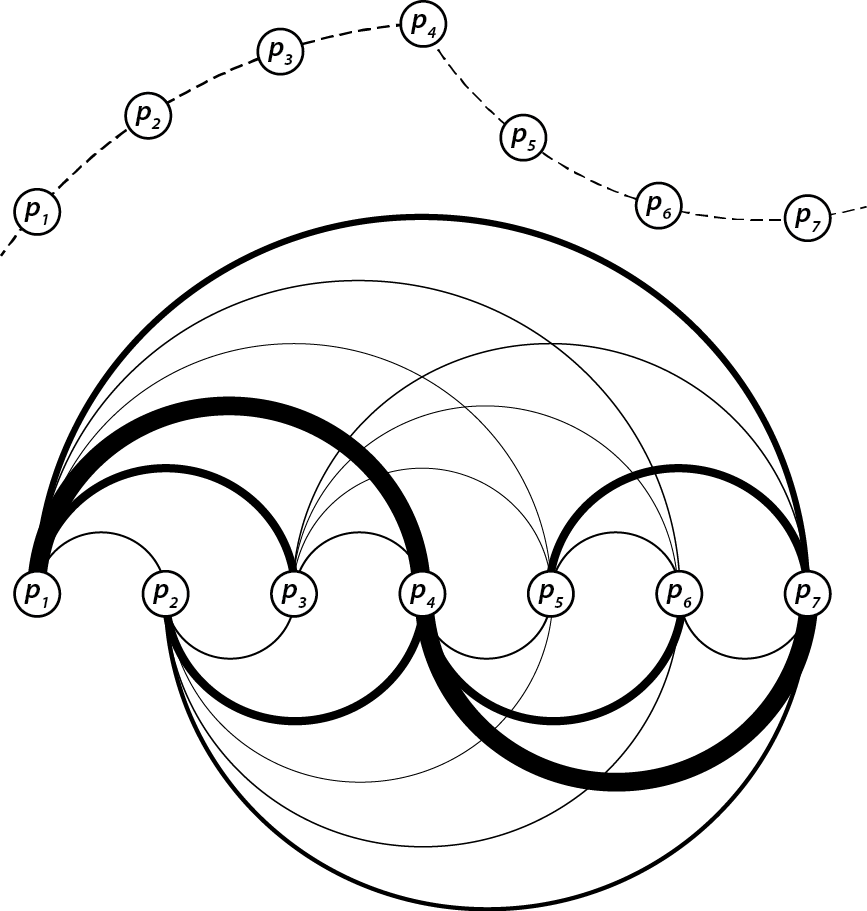
\includegraphics[scale=0.6]{graph.png}

\caption{\small An APWP (upper panel) seen as a graph (lower panel) where the thickness of the lines (edges) connecting pairs of poles (nodes) is inversely proportional to the cost of traversing the path (weight).}

\label{fig:graph}
\end{centering}
\end{figure}

In graph or network theory, Dijkstra's algorithm allows identification of the shortest path between two given nodes \citep{dijkstra1959note}, such that the sum of the weight of its constituent edges is minimized. In an ideal (noiseless) case, the sum of the weight of its constituent edges connecting the youngest node and the oldest one, is null. We perform shortest path searches through the open-source package SciPy \citep[scipy.sparse.csgraph.shortest\_path,][]{virtanen2020scipy}. 

The hyperparameter $\lambda$ is adjusted to improve the accuracy of the model to avoid overfitting, namely, by preventing an over-estimation of the number of segments, $m$. We apply the 'Elbow' method to find the $\lambda$ value that yields the optimum value of $m$  \citep{bholowalia2014ebk}. This is achieved by plotting the total cost against the number of segments $m$ and evaluating their tradeoffs: (too) small values of $m$ will add large total costs but at some threshold value of $m$ the cost will be observed to decrease sharply. Above this threshold, further increasing $m$ will not yield significant further reductions to the total cost. The graphical 'elbow' in the plot thus points to this optimal value of $m$.

We summarize our algorithm to find the optimal sequence of Euler vectors to approximate a given sequence of paleomagnetic poles $P$ as follows:

\begin{enumerate}
    \item For each time-ordered  pair of paleomagnetic poles $p_i$ and $p_j$, find the circle in $P_{i-j} = \{ p_i, \ldots, p_{j} \}$ that minimizes the value of $\mathcal C_{i-j}$ plus $\lambda$.
    \item Construct a directed graph and select $\lambda$ through the Elbow method to avoid overfitting.
    \item Use Dijkstra's algorithm to find the shortest path between the first pole $p_1$ and the last pole $p_N$. 
    \item From the optimal path, we recover the parameters of the stage Euler vectors for each APWP segment.
\end{enumerate}

\section{Results}

To illustrate the application of our methodology, we execute a simple test involving idealized synthetic paleomagnetic data.  We start by generating a stochastic model of the drift of a plate over 200 Myr by randomly generating stage Euler vectors---represented in the matrix form as $R(q,\omega)$---which remain constant during a temporal stage of given duration. The geographic coordinates of each Euler vector $(\theta_{q}, \phi_{q})$ are randomly selected from a uniform distribution on the unit sphere and their angular velocities $\omega$ are chosen from a uniform distribution constrained between 0.5$^{\circ}$/Myr and 2.5$^{\circ}$/Myr (which yields plate velocities up to ~28 cm/yr). The corresponding duration of each Euler vector is randomly selected from a uniform distribution between 10 and 30 Myr, and Euler vectors are drawn until their summed durations reach or exceed 200 Myr. Using this stochastic kinematic model, we assemble a synthetic APWP populated by paleomagnetic poles every 1 Myr (Figure \ref{fig:figure4}a). To replicate a more realistic scenario with noise, we perturb the geographic coordinates of the paleomagnetic poles by Gaussian random noise up to 0.1$^{\circ}$. Note that the latter step is only taken to demonstrate the capacity of our method to handle noise; a more comprehensive consideration of the feasibility of PEP given standard paleomagnetic noise has yet to be addressed.


Next, we proceed to invert the synthetic paleomagnetic data according to the methodology outlined above. First, for each candidate APWP segment (all ordered subsets of the paleomagnetic data) we compute the best-fitting Euler vector by minimizing equation \eqref{eq:cost_3}. We then organize the computed costs as a graph in the form of an adjacency matrix, which can be rendered visually as a heatmap (Figure \ref{fig:figure4}b). Visual inspection of this heatmap reveals strong contrasts in the magnitude of the cost function, which tends to increase sharply with the passage of a change-point. Using the regularization introduced in equation \eqref{eq:cost_3} and the Elbow method (Figure \ref{fig:figure4}c), we identify the shortest path through this graph following Dijkstra's algorithm, which yields the number of segments $m$ and a discrete set of change-points $(j_1, j_2, \ldots, j_{m+1})$. From this sequence of change-points, we retrieve the parameters of the minimum circle $\Theta^{(k)}$ for each segment $P_{j_k - j_{k+1}}$, enabling us to infer the complete kinematic history through the series of stage Euler vectors $\hat R (q,\omega)$. The workflow can be run interactively in the browser via \textit{Binder} (\url{https://mybinder.org/v2/gh/LenGallo/PEPy/HEAD}) with a synthetic example in the Jupyter Notebook (APWP.ipynb).

\begin{figure}
\begin{centering}
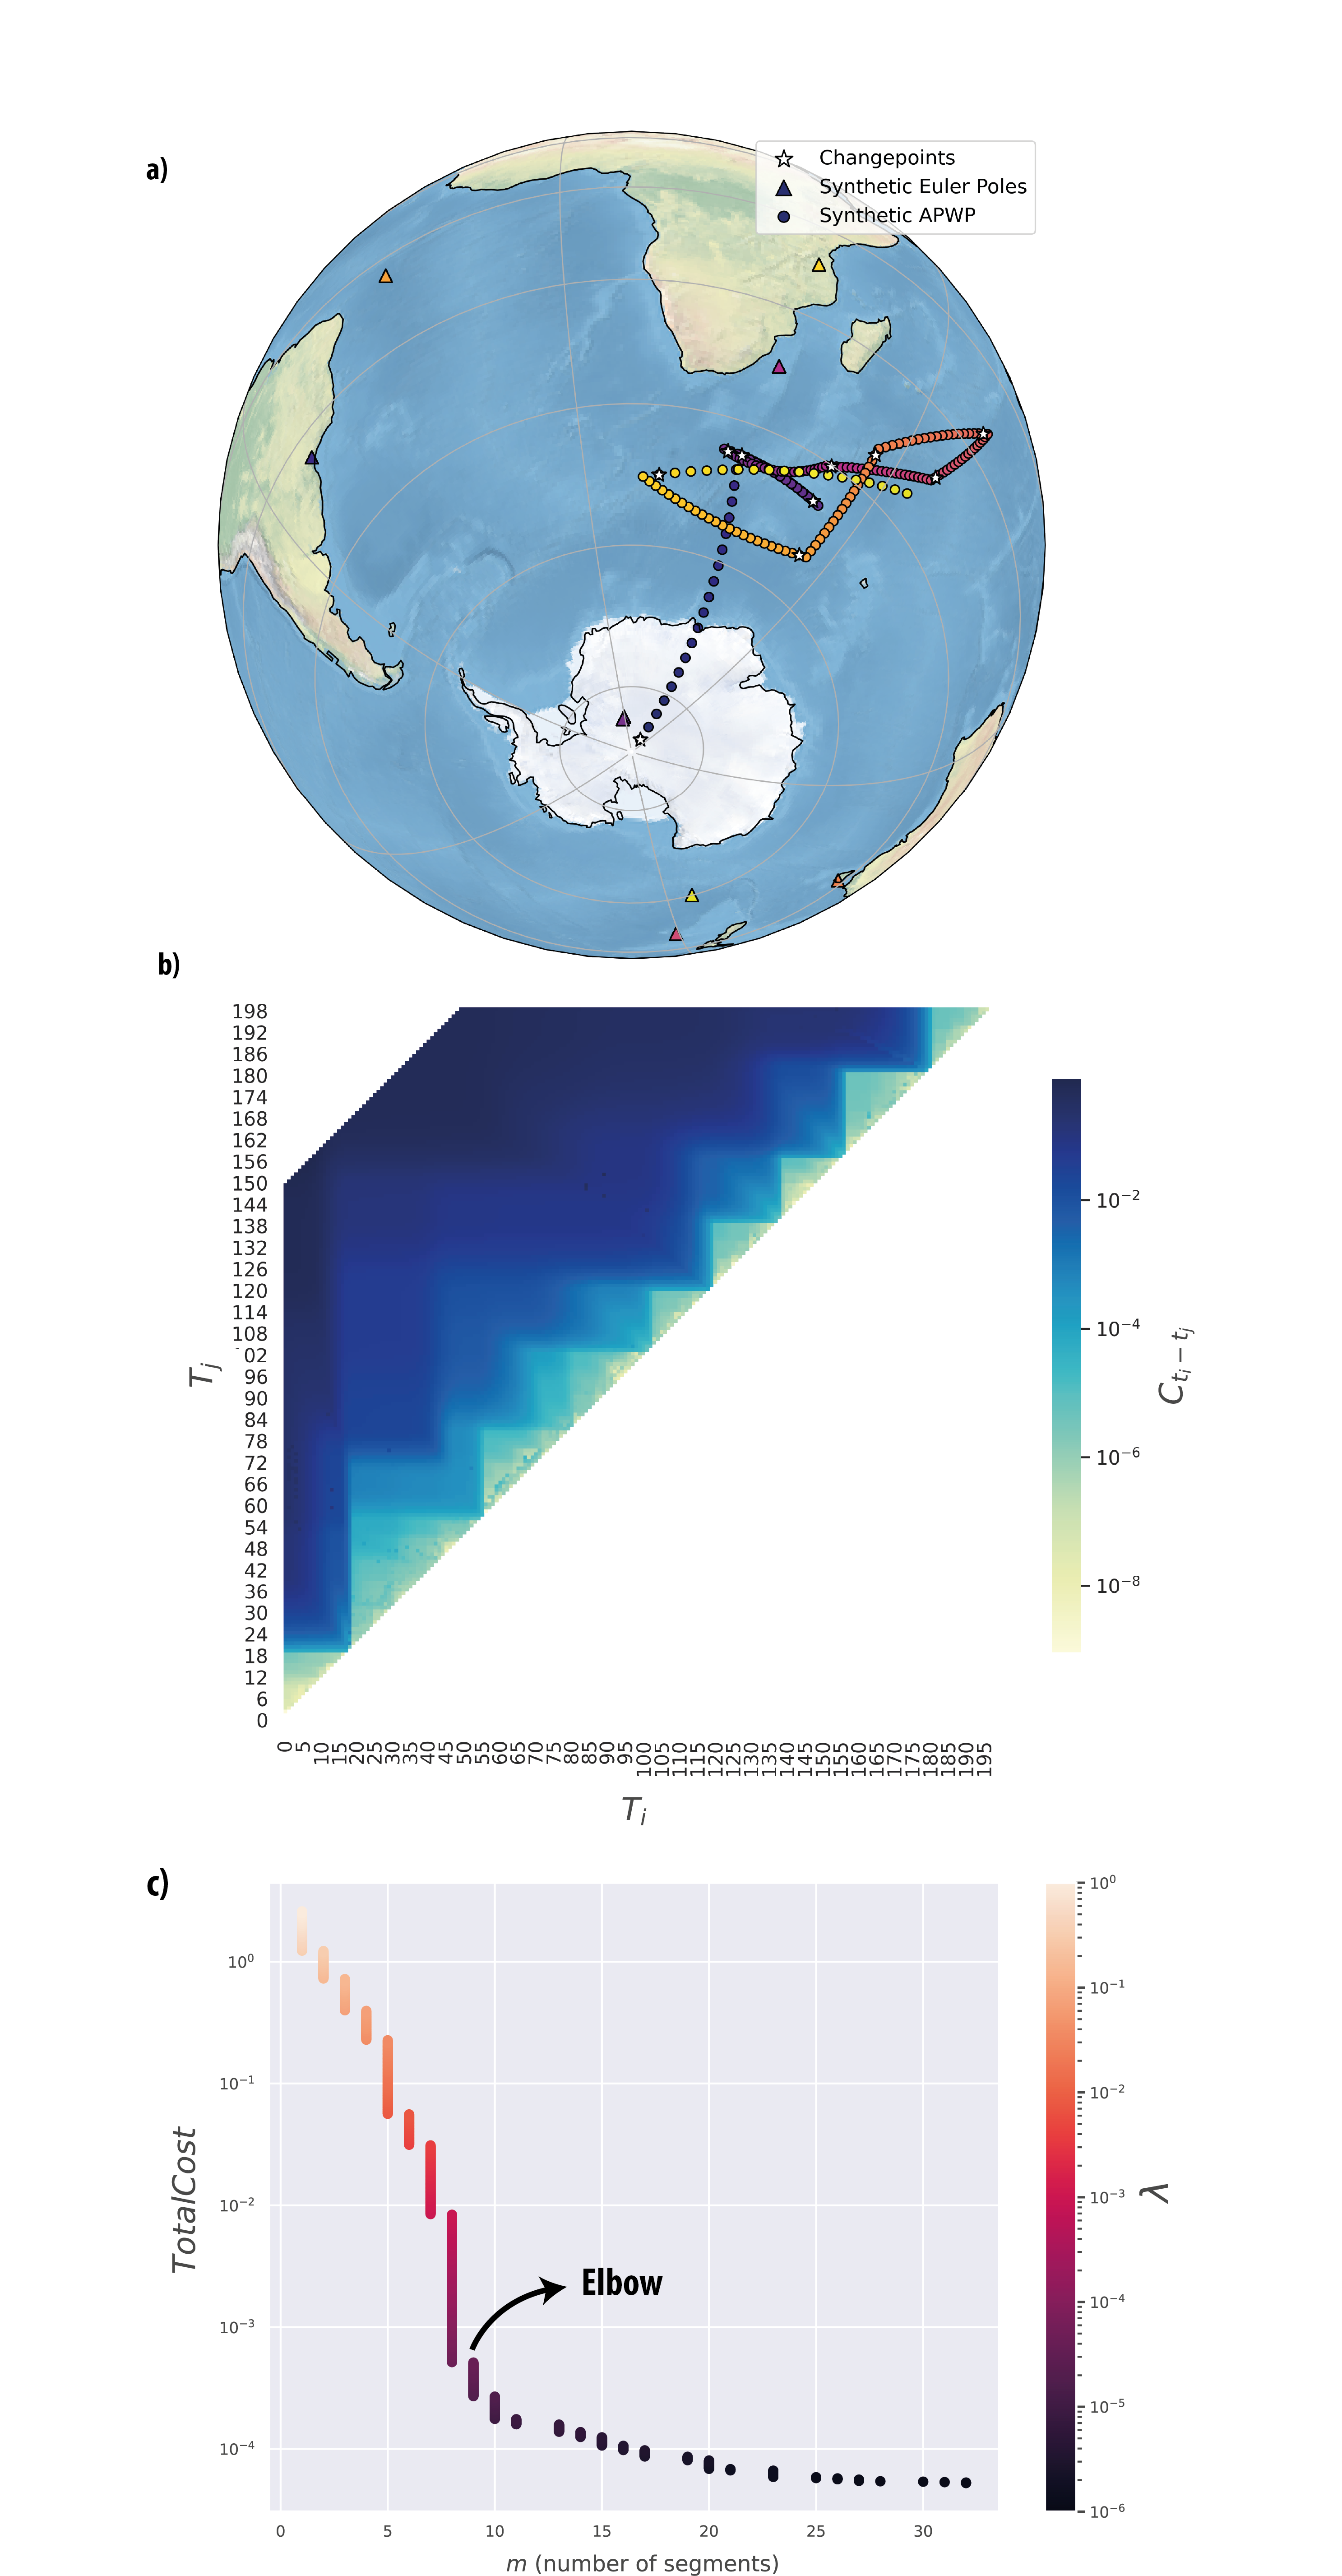
\includegraphics[scale=0.4]{Figure 4.png}

\caption{\small Graphical illustration of the application of our methodology. a) We start by generating a stochastic model of the drift of a plate over 200 Myr by randomly generating stage Euler vectors (triangles). From this stochastic kinematic model, we assemble a synthetic APWP (dots) populated by paleomagnetic poles every 1 My. b) Heatmap visualization of the adjacency matrix illustrating the magnitede of the cost function for each candidate APWP segment. c) Scatter plot illustrating the Elbow method: the total cost (y axis) is plotted against the number of segments $m$ (x axis), color coded by the hyperparameter $\lambda$. The graphical 'elbow' in the plot thus points to this optimal value of $\lambda$.}

\label{fig:figure4}
\end{centering}
\end{figure}

To measure the performance of our graph-based PEP methodology in terms of accuracy, we generate 1000 stochastic models of the drift of plate
%---a number large enough to allow us to draw statistically meaningful inferences---
and invert the paleomagnetic data from each for the series of underlying stage Euler vectors $\hat R (q,\omega)$. Comparisons between the pairs of true $R (q,\omega)$ and estimated $\hat R (q,\omega)$ stage Euler vector series are then assessed by a variety of metrics. Using the inverted kinematic model, we assemble a synthetic APWP and compute the time-dependent geodesic distance (i.e. residual) between it and the known APWP. In Figure \ref{fig:ensemble}a we show the ensemble median of this residual, along with the 0.25-75 and 0.16-0.84 percentile ranges representing standard confidence intervals. As could be expected, we observe that average misfits tend to accumulate backward in time, but we note that they never exceed 3 degrees. In \ref{fig:ensemble}b-c we further dissect the discrepancies: in panel b we show the ensemble median of the time-depedendent geodetic distance between Euler poles, while panel c shows the difference in angular velocities. These results reveals that the average misfit between the true and estimated stage Euler vectors of any given simulation is low. 
Furthermore, we compare the true kinematics and our inferences quantifying the discrepancy of the drift of a given point after rotation by the series $R$ and $\hat{R}$. We start by generating 5 nodes evenly distributed in latitude (in the central meridian) and we then calculate a time-dependant geodesic distance between the inferred drift and the true drift for each point. Last, we compute the mean of these distances for each time in order to illustrate the time-dependant drift (i.e. total motion) misfit. Figure \ref{fig:ensemble}d shows that the median of the drift misfit never exceeds 4 degrees. Finally, we address the velocity surface misfit associated with our kinematic inferences. With that aim, the surface velocity at each of the former points is calculated through the cross-product between each one of the former points and the true and inferred Euler vectors.

Considering all these ensemble medians to be representative of the misfit associated with the workflow in the absence of significant noise, we conclude from these metrics that our methodology can robustly retrieve the kinematics of a plate from its APWP.


\begin{figure}
\begin{centering}
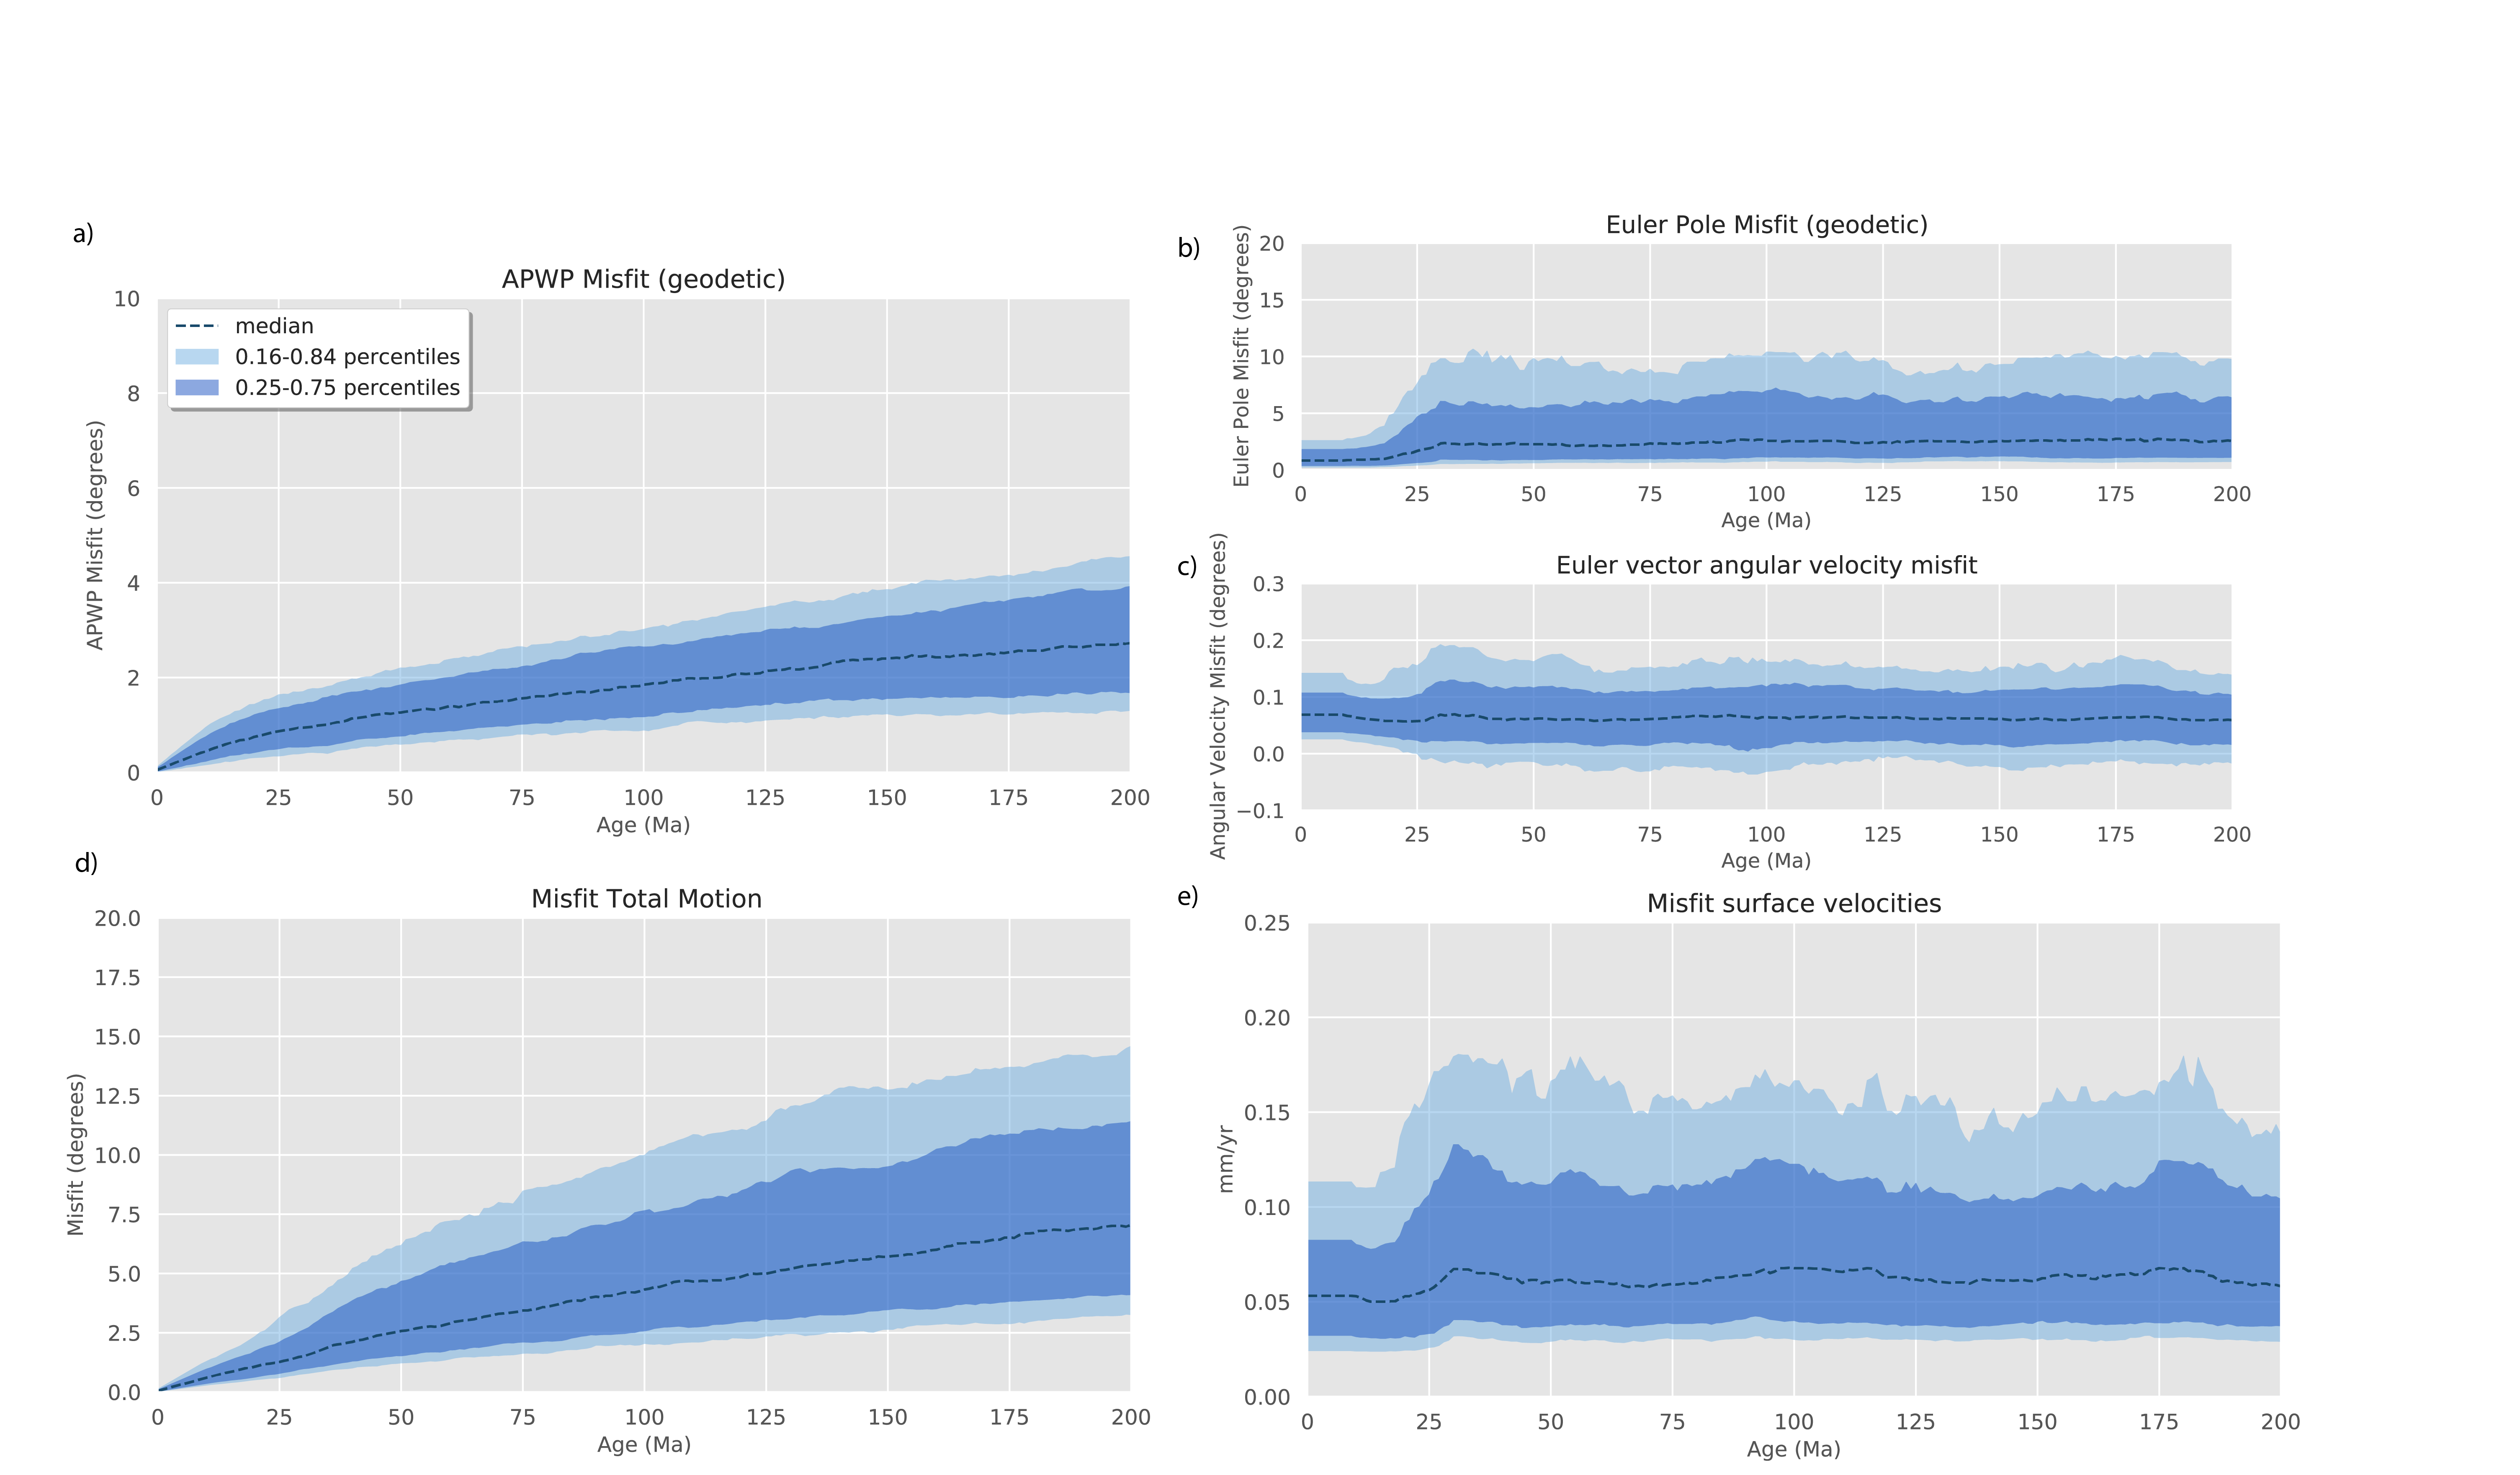
\includegraphics[scale=0.35]{ensemble-statistics.png}

\caption{\small Ensemble statistics of 1000 stochastic models of the drift of a plate for the comparison between the pairs of true kinematics and those inverted from our graph-based PEP methodology. The dashed line represent the ensemble median along with the 0.25-75 and 0.16-0.84 percentile ranges representing standard confidence intervals. a) Geodesic time-dependant distance between the known APWP and the assembled using the inverted kinematic model. b) Time-depedendent geodesic distance between Euler poles. c) Difference in angular velocities of the true and inverted Euler vectors. d)  Mean discrepancy of the drift of 5 points evenly distributed in latitude after rotation by the series $R$ and $\hat{R}$. e) Velocity surface misfit associated with our kinematic inferences.}

\label{fig:ensemble}
\end{centering}
\end{figure}

\section{Discussion}

%Reflections on previous work and the improvements herein..
Conceptually, in providing a means to retrieve the full kinematic histories of tectonic plates from paleomagnetic data, PEP analysis presents an enormously powerful tool. And yet, despite its foundations being laid more than half a century ago \citep{francheteau1969paleomagnetism}, lingering doubts about the rigor and viability of PEP analysis have left it largely stranded in obscurity.

%Firstly, although our approach to fitting small circles to a set of paleomagnetic data is underpinned by the same fundamental minimization used by all previous studies, our use of the gradient-descent method to solve this problem is far more efficient than the undirected grid search employed by some of those previous efforts \citep[e.g.][]{gordon1984paleomagnetic}. This increased efficiency is not only important in facilitating the remainder of our algorithm (identifying the least-cost pathway of an APWP), but also lays the groundwork for handling real (e.g. noisy) paleomagnetic data (see below). However, the most significant advancement presented herein is the objective identification of change-points and the automated inversion of the corresponding APWP segments to infer full plate kinematic histories from paleomagnetic data. 
One of the most significant and persistent shortcomings in PEP analysis has been the subjective determination of which APWP segments to invert, and which inversions to retain. As noted by previous studies \citep[e.g.][]{tarling1996palaeomagnetic,wu2014derivation}, the optimal fits to real paleomagnetic data tend toward short segments associated with proximal circles of small-radii, which together often imply improbable rates of plate motion change, unrealistic angular velocities and/or geologically dubious kinematics. As a consequence, the selection of which segments to fit has been done \textit{a priori} by visual inspection \citep[e.g.][]{gordon1984paleomagnetic,may1986north,wu2014derivation}, undercutting the rigor and reproducibility of the analysis. In some instances the best-fitting small-circle solutions have also been dismissed in favor of either subjective assessments of more feasible solutions \citep{tarling1996palaeomagnetic} or forced great-circle fits \citep{smirnov2010co}. Although \cite{smirnov2010co} consider the use of great-circle fits to be a conservative measure, we note that approach confines all stage Euler vectors to the equatorial plane. \cite{RosePhdthesis} presented a significant step forward in introducing a Bayesian approach to PEP analysis (later applied by \cite{swanson2019failed}), which addressed some of these issues of subjectivity and presented a pathway toward a more comprehensive treatment of uncertainty in such analyses. However, in its present formulation, their approach still regularize the problem through the choice of the number of change-points.

Our methodology addresses several of these deficiencies, and notably the problem of objectively selecting change-points, by identifying the least-cost solution without supervision. The least-cost solution is a full approximation of the APWP, such that the location of the change-points and the parameters of the stage Euler vectors defined between them are fully and automatically determined by the algorithm. Although the method employs a regularization parameter to avoid overfitting, the Elbow method allows a more  objective selection of this parameter. Other parameters that can be modified by the user (number of inversion seeds, maximum duration of a given stage)---while capable of affecting the outcome if set to too low values---are used to improve efficiency and so can be set to arbitrarily high values. Admittedly, our experiments here have been conducted on idealized synthetic data, and it can be anticipated that experiments with real (noisy) data may introduce circumstances in which the least cost solution can otherwise be shown to be unrealistic (e.g. requiring impossibly high rates of rotation). However, the flexibility of our methodology is such that minor adaptions to our optimization framework (e.g. specifying constraints to rotation rates in the optimization problem) allow such issues to also be tackled systematically.

%Things that remain to be done with PEP..
Despite the advancements presented herein, there remain a number of significant challenges associated with the application of PEP analysis to real paleomagnetic data. The first is the feasibility of the methodology in light of the noise accompanying paleomagnetic data, arising from both intrinsic (geomagnetic secular variation) and extrinsic (e.g. age uncertainties, tectonic rotations, inclination shallowing) uncertainties. Although the cost function can be further constrained to avoid unrealistic solutions, there exists some level of noise above which the uncertainty in the solution space is so vast that the optimal solution is rendered meaningless. However, a systematic exploration of these noise thresholds, as well as the trade-offs between noise level and the rate of plate motion, have yet to be conducted. 

A second challenge concerns the phenomenon of true polar wander (TPW). TPW is a rotation of the entire solid Earth which occurs in response to changes in the planetary moment of inertia following changes to Earth's internal distribution of mass \citep{goldreich1969some}. Because TPW always acts to restore the largest inertial axis to the planetary axis of rotation, TPW always occurs about an equatorial axis. Thus, during a TPW event, the entire tectonic plate system (together with the mantle) will move relative to the spin axis by a common angular displacement. Paleomagnetic data, in recording the movement of the lithosphere relative to the magnetic field (which remains parallel to the spin-axis during TPW) therefore represents some composite signal of TPW and individual plate motion. Before PEP analysis can be applied to any given paleomagnetic dataset, the TPW signal needs to be removed from it. Unfortunately, time-dependent estimates of TPW are themselves uncertain and often controversial. More significantly, prior to Cretaceous time, TPW estimates are derived from plate kinematic models \citep{steinberger2008absolute}; any results from PEP analysis employing these TPW estimates would thus undermine their own foundation wherever they challenged the underlying kinematic model. Future progress on this front will likely necessitate a joint modelling approach.  

We end with a reminder that the methodology and tools presented herein, while motivated by the desire to improve upon existing approaches in PEP analysis, are not restricted to paleomagnetic applications. They could, for example, be equally applied to hotspot tracks. There are also broader applications of the small-circle fitting operation (which is intentionally presented as a standalone tool), as arise, for example, in structural geology (supplementary materials figure?).

\section{Conclusions}

Owing to the inherent axial symmetry of the Earth’s magnetic field, paleomagnetic data only directly record the latitudinal and azimuthal positions of crustal blocks in the past, but paleolongitude cannot be constrained. The paleomagnetic Euler pole concept presents a unique means by which to estimate motions in deep-time. We have presented a methodology that enables PEP analysis to be conducted in a fully data-driven way. Our methodology follows the solution of two distinct optimization problems. We first find the parameters of the best-fitting circle to a set of paleomagnetic poles through a gradient-based Euler vector optimization method. Then, through an exploratory data analysis, all the possible segments at every point of the APWP are assessed in order to transform the data into a weighted, undirected graph. This graph representation of the APWP allows the identification of that sequence of stage Euler vectors which together present the least cost (shortest path of the graph) description of an observed APWP. We demonstrated the performance of our algorithm with a set of simple experiments with synthetic data drawn from stochastic kinematic histories, from which our inversions recovered kinematic parameters that closely resembled the known values. We closed with a discussion of some challenges that remain for the application of PEP analysis to real paleomagnetic data, and a note that the tools presented herein have applications beyond PEP analysis.

%We have presented a methodology that enables PEP analysis to be conducted in a fully data-driven way. Our methodology follows the solution of two distinct optimization problems: firstly the parametrization of the best-fitting circle to a set of paleomagnetic data, and secondly the identification of that sequence of stage Euler vectors which together present the least cost (shortest path) description of an observed APWP. This formulation thus allows the individual stage Euler vectors and the change-points separating them to be discovered systematically. We demonstrated the performance of our algorithm with a set of simple experiments with synthetic data drawn from stochastic kinematic histories, from which our inversions recovered kinematic parameters that closely resembled the known values. We closed with a discussion of some challenges that remain for the application of PEP analysis to real paleomagnetic data, and a note that the tools presented herein have applications beyond PEP analysis.

\section{Acknowledgments}

This project has received funding from the European Union’s Horizon 2020 research and innovation program under the Marie Skłodowska-Curie grant agreement No. 101025975 (L.C. Gallo) and from the Research Council of Norway through the Centres of Excellence funding scheme, project number 22327. The simulations were performed on resources provided by UNINETT Sigma2 - the National Infrastructure for High Performance Computing and Data Storage in Norway.


%%%%%%%%%%%% Supplementary Methods %%%%%%%%%%%%
%\footnotesize
%\section*{Methods}

%%%%%%%%%%%%% Acknowledgements %%%%%%%%%%%%%
%\footnotesize
%\section*{Acknowledgements}

%%%%%%%%%%%%%%   Bibliography   %%%%%%%%%%%%%%
%\normalsize
%\bibliographystyle{apacite}
\bibliography{references}

%%%%%%%%%%%%  Supplementary Figures  %%%%%%%%%%%%
%\clearpage

%%%%%%%%%%%%%%%%   End   %%%%%%%%%%%%%%%%
%\end{multicols}  % Method B for two-column formatting (doesn't play well with line numbers), comment out if using method A
\end{document}
